\chapter{MultiChannel Analyzer}
\section{Analisi degli impulsi con un MCA}
Lo spettro \`e una funzione $\frac{dN}{dH}$, nella realt\`a \`e nella forma $\frac{\Delta N}{\Delta H}$, con $\Delta H$ larghezza di un canale.\\
In passato l'analisi di uno spettro avveniva con un SCA le cui soglie venivano regolate di volta in volta, adesso questi studi vengono effettuati
utilizzando degli SCA in parallelo, ovvero con un MCA.
Lo svantaggio nell'uso di un MCA \`e nella possibile sovrapposizione di canali, oppure nella non perfetta uniformit\`a delle loro larghezze.
\section{Caratteristiche di un MCA}
\subsection{Canali richiesti}
Il numero di canali richiesti per un'analisi \`e importante, esso \`e determinato da tre fattori:
\begin{itemize}
\item Risoluzione del rivelatore
\item Binning del software di analisi
\item Conteggi per canale
\end{itemize}
Lo spettro discreto deve essere il pi\`u possibile vicino a quello continuo, tuttavia aumentare troppo il numero di canali
riducendo la loro larghezza ha degli inconvenienti: essendo la statistica a singolo canale di tipo poissoniana, restringere un canale
riduce il numero di conteggi, quindi la loro fluttuazione cresce (va come l'inverso del numero di conteggi), nascondendo l'eventuale
presenza di picchi secondari deboli (fig.~\ref{fig:binningMCA}). 
\begin{figure}[htbp]
\begin{center}
	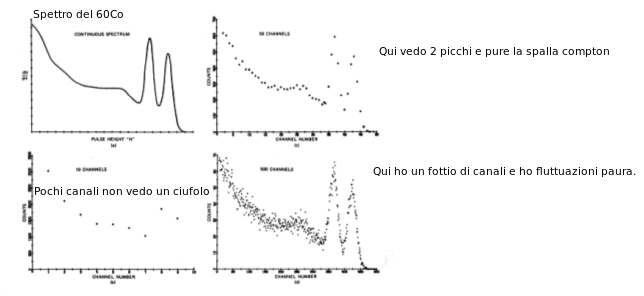
\includegraphics[scale=0.7]{./Immagini/BinningMCA.png}
\label{fig:binningMCA}
\end{center}
\end{figure}
In genere i software di analisi richiedono 9-12 canali corrispondenti alla FWHM\%, per cui a una FWHM\% del 10\% corrispondono circa 100 canali nel picco.
\subsection{Calibrazione e linearit\`a}
In un MCA ideale, la retta di calibrazione canale-tensione \`e perfettamente lineare; nella realt\`a questo non accade, in generale \`e possibile
aggiungere degli offset per fare in modo che al canale 0 corrispondano tensioni non nulle.
La pendenza della retta di calibrazione tensione-canale \`e dipendente dall'elettronica, ad esempio cambiare l'amplificazione modifica la sua pendenza,
se il dispositivo \`e lineare, sono sufficienti due punti per ottenere il fit, nella realt\`a questa calibrazione viene fatta con molti pi\`u punti, 
in modo da testare la linearit\`a.\\
Ho due tipi di non-linearit\`a: quella integrale, che mi da la massima deviazione tra la tensione sperimentale del canale e la curva best fit;
quella differenziale, ottenuta sottoponendo l'MCA ad una distribuzione uniforme in ampiezza di impulsi ed acquisendone lo spettro, in modo
da determinare disuniformit\`a nella larghezza del canale.
Un buon MCA ha deviazioni di non linearit\`a differenziali nel \%.
\begin{figure}[htbp]
\begin{center}
	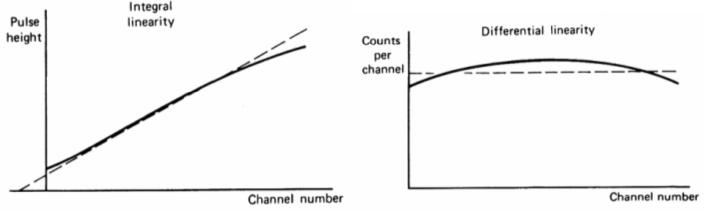
\includegraphics[scale=0.60]{./Immagini/NonLinearitaMCA.png}
\caption{Curve di non linearit\`a in un MCA}
\end{center}
\end{figure}
Una possibile sorgente di non linearit\`a viene anche dall'ADC che come gi\`a visto pu\`o avere larghezze dei canali non omogenee.
\section{Componenti di un MCA}
Il cuore di un MCA \`e dato dall'ADC (non di tipo flash o multipasso), esso riceve il segnale e ne digitalizza il picco.
Prima di un ADC \`e presente un circuito di ingresso, esso ha lo scopo di trattenere in memoria l'impulso e trasmetterlo all'ADC per tutta la durata della conversione,
un gate blocca tutti gli impulsi per la durata della conversione e da informazioni sul tempo morto del MCA.
All'uscita del ADC \`e presente una memoria formata da tante regioni quanti i canali del ADC e che conteggia il numero di segnali ricevuti, in genere
il numero di bit per area di memoria \`e tale da poter tenere un numero di conteggi nell'ordine dei $10^9$.\\
Spesso all'ingresso di questa catena viene posizionato un SCA, esso viene utilizzato per selezionare impulsi contenuti in una particolare regione,
in questo modo \`e possibile ridurre il tempo morto del MCA non facendo digitalizzare gli impulsi non utili.\\
Al termine della catena \`e presente un terminale che visualizza i dati e li salva, spesso si utilizza un PC. 
Il PC, tuttavia, \`e un ambiente rumoroso, per cui \`e necessario avere un architettura dedicata oppure posizionare l'ADC esternamente al dispositivo.
\section{Dettagli sul ADC}
Come detto prima, ADC flash e multipasso hanno problemi di non linearit\`a, per questo si usando altri tipi di ADC.
\subsection{ADC con rampa lineare (Wilkinson)}
In questo ADC all'arrivo del segnale viene prodotta, mediante una corrente costante ed un condensatore, una rampa lineare.
Un impulso di gate rimane attivo per il periodo di tempo in cui la rampa \`e sotto la tensione in ingresso e viene utilizzato
per pilotare degli impulsi di clock.
Il numero di impulsi di clock indica quanto tempo il gate \`e rimasto attivo e quindi il numero di impulsi prodotti sono una digitalizzazione
del segnale.
Chiaramente in questo ADC il tempo di digitalizzazione dipende dall'ampiezza dell'impulso ed \`e nell'ordine di multipli del reciproco della frequenza di clock,
frequenze tipiche sono nel centinaio di MHz (10 ns per canale), ma ha il vantaggio di avere un'ottima linearit\`a.
\subsection{ADC ad approssimazioni successive}
Questo ADC si basa su una sorta di ricerca dicotomica, un comparatore compara il segnale con la tensione corrispondente al 
primo bit pi\`u significativo del ADC. 
Se \`e maggiore allora il bit pi\`u significativo viene posto a 1 e si sottrae la tensione corrispondente al segnale originale, altrimenti esso viene posto a 0.
Il segnale viene quindi passato ad uno stadio che esegue lo stesso lavoro con il secondo bit pi\`u significativo e cos\`i via.\\
Il vantaggio di questo dispositivo \`e che ha tempi di conversione costanti (se ho 10 bit faccio 10 passaggi con tempi nei microsecondi), tuttavia ha non linearit\`a maggiori.
\subsection{Il principio della scala che scorre}
Questo metodo permette di ridurre le DNL, una tensione casuale viene aggiunta al segnale che viene successivamente digitalizzato.
La stessa tensione aggiunta viene anch'essa digitalizzata e poi sottratta al output del primo segnale.
Supponendo che alla tensione casuale corrisponda il canale M e che le fluttuazioni sulle larghezze dei canali siano casuali, questo metodo
migliora le uniformit\`a dei canali di un fattore $\sqrt{M}$.\\
Il problema principale di questo metodo \`e che se si suppone di dare pi\`u volte lo stesso segnale in ingresso esso pu\`o corrispondere a canali differenzi
con un peggioramento della risoluzione del MCA (senza il metodo avremmo tutto nello stesso canale, in proporzione alla sua DNL).\\
Un altro problema \`e dato dall'utilizzo di due ADC diversi: se i fattori di scala non sono bene accoppiati possono apparire strutture artefatte nello spettro.
\section{Tempo morto degli MCA (NON HO CAPITO IL METODO HARMS)}
Le sorgenti principali di tempo morto all'interno di un MCA sono due: l'ADC e la memorizzazione.
\`E importante misurare il tempo morto per poterlo successivamente correggere.\\
Per MCA con ADC Wilkinson il tempo morto segue la relazione:
\begin{equation*}
\tau = \frac{N}{\nu}  + B
\end{equation*}
con $N$ canale dell'impulso, $\nu$ frequenza del clock del ADC e $B$ tempo di memorizzazione.
In genere il tempo morto non dovrebbe superare il 30-40\% del tempo totale, altrimenti si possono osservare deformazioni dello spettro.\\
Gli MCA possiedono delle componenti che si occupano di misurare il tempo morto del dispositivo osservando la presenza del gate; questi misuratori sono affidabili purch\'e il tempo morto
non sia troppo elevato, altrimenti \`e necessario ricorrere ad altri metodi.\\
Un metodo \`e utilizzare un impulsatore per produrre impulsi artificiali nel PRE che verranno successivamente formati ed acquisiti.
Nel MCA ci si aspetter\`a di osservare un picco artificiale di una cerca area, osservando il rapporto tra gli impulsi acquisiti e gli impulsi prodotti si pu\`o determinare
il tempo morto; gli impulsi non devono essere prodotti troppo frequentemente e talvolta \`e preferibile utilizzare una produzione casuale.
Questo metodo \`e buono se lo spettro del MCA non ha derive nel guadagno o variazioni nei rate di misura, altrimenti pu\`o incorrere in problemi.\\
Un metodo suggerito da Harms \`e quello di produrre impulsi per un tempo di clock fissato.
\`E possibile determinare quando un impulso \`e stato perso esternamente (quindi dedurre il tempo morto),
in questo caso il tempo morto verr\`a compensato dando all'impulso successivo peso doppio.
Osservando lo spettro prodotto da tali impulsi \`e possibile determinare eventuali derive nello spettro. 
In caso di alti rate, il metodo pu\`o essere esteso conteggiando gli impulsi persi e aumentando del relativo fatto il peso dell'impulso successivo.
\section{Stabilizzazione dello spettro}
Eventuali derive dello spettro possono deformare i picchi, rendendo difficili le analisi spettrali.
Le cause di queste derive sono molteplici: variazioni di temperatura, di tensione, di guadagno, del tasso di conteggi (soprattutto negli scintillatori).\\
Gli stabilizzatori di spettro si occupano di percepire tali derive e correggere lo spettro di conseguenza. 
Una tecnica utilizzata \`e quella di porre due SCA simmetrici rispetto ad un picco e conteggiare il numero di impulsi, in assenza di derive il conteggio
sar\`a simmetrico, altrimenti sar\`a sbilanciato verso una coda, permettendo di misurare e correggere derive nel guadagno;
questa tecnica pu\`o essere applicata digitalmente utilizzando due Range Of Interest (ROI) nello spettro del MCA.
Questa tecnica pu\`o essere utilizzata ogni tot impulsi e correggendo di conseguenza, il problema \`e che statisticamente gli spettri sono sempre asimmetrici,
per cui ci sar\`a sempre una correzione nel guadagno, peggiorando la FWHM del picco. 
Tuttavia, se le fluttuazioni statistiche sono piccole, questo effetto pu\`o essere trascurato.\\
\`E inoltre possibile correggere offset utilizzando due picchi all'inizio e alla fine dello spettro.\\
Gli impulsi di test possono venire da una sorgente, oppure da un impulsatore, tuttavia quest'ultimo permette di testare unicamente l'elettronica, ma non lo scintillatore.
Utilizzare una sorgente pu\`o comportare del fondo indesiderato.
\subsection{Riallineamento dello spettro}
Un modo per risolvere il problema della deriva dello spettro \`e suddividere la misura in misure pi\`u brevi.
Il problema, comunque, rimane in quanto per avere una statistica maggiore pu\`o essere utile unire nuovamente gli spettri.
Questi spettri avranno un binning e una calibrazione diversa di volta in volta.\\
Il primo passo per affrontare il problema \`e quello di utilizzare pi\`u picchi per spettro, in modo da poter calibrare i singoli spettri e riportarsi sulla scala delle energie.
A questo punto \`e necessario utilizzare un binning comune in energia, per cui \`e necessario effettuare un rebin degli istogrammi per renderli tutti uniformi.\\
Supponiamo di voler rebinnare una regione di $M$ canali, se essi sono piccoli \`e possibile interpolarli con una polinomiale di grado $M-1$ per ottenere lo spettro continuo.
A questo punto, eseguendo il rapporto tra le aree sottese dalla polinomiale nel bin finale e quello originale, \`e possibile suddividere i vari bin sulla base del rapporto ed ottenere un buon rebinnaggio dei dati.
Questo metodo, tuttavia, fa perdere la statistica poissoniana dei singoli bin.
\section{Analisi degli spettri}
\subsection{Deconvoluzione e ricostruzione dello spettro reale}
Quando misuriamo uno spettro quello che viene osservato non \`e il vero spettro, in quanto l'elettronica risponde in modo diverso a seconda degli impulsi,
in particolare lo spettro osservato pu\`o essere scritto come:
\begin{equation*}
\frac{dN}{dH} = \int S(E) R(H,E) dE
\end{equation*}
dove $S(E)$ \`e lo spettro reale, mentre $R(H,E)$ \`e la funzione di risposta ovvero la probabilit\`a che un quanto di energia $E$ produca un impulso di ampiezza $H$.\\
Se supponiamo di avere una sorgente ad energia fissata, allora lo spettro reale \`e una delta di ampiezza $S_0$ e l'espressione precedente risulta:
\begin{equation*}
\left.\frac{dN}{dH}\right|_{E=E_0} = S_0 \, R(E_0,H)
\end{equation*}
Nel caso di un MCA si lavora con spettri discreti, quindi l'integrale diventa una sommatoria:
\begin{equation*}
N_i = \sum_{j} S_j R_{ij}
\end{equation*}
con $N_i$ numero di conteggi al canale i-esimo, $S_j$ ampiezza dello spettro (quindi l'intensit\`a di radiazione) all'energia j-esima, $R_{ij}$ matrice di risposta del sistema.\\
Lo spettro reale \`e chiaramente un continuo, ma dato che lo vediamo discreto, possiamo discretizzarlo in $L$ intervalli;
allora se conosco $R_{ij}$ posso risolvere il sistema associato e trovare $S_j$: avendo M canali, quindi M equazioni, il sistema \`e risolvibile per $L\le M$,
effettuando cos\`i la \textbf{deconvoluzione dello spettro}.
Se $R(H,E_0) = R_0 \delta (H-H_0)$ allora la matrice \`e diagonale ed esiste una corrispondenza biunivoca tra gli spettri, ma questo non capita sempre.\\
La tecnica della deconvoluzione possiede diversi problemi: inanzitutto non \`e possibile conoscere con precisione $R_{ij}$ in quanto non \`e possibile provare
la risposta ad ogni singola energia; inoltre anche conoscendo tutte le energie esistono problemi di natura statistica legati alla varianza di un singolo bin e
al fatto che le condizioni di lavoro possono cambiare.
Per questi motivi non \`e possibile conoscere con precisione lo spettro $S_j$, ma ci si accontenta di soluzioni approssimate,
un modo \`e quello di minimizzare la funzione di somma pesata dei residui:
\begin{equation*}
\epsilon^2 = \sum_i W_i \left(N_i - \sum_j S_j R_{ij}\right)^2
\end{equation*}
con $W_i$ pesi inversamente proporzionali all'incertezza del residuo. 
Per ridurre le incertezze si pu\`o eseguire del data smoothing, ovvero si pu\`o eseguire una media pesata dei canali con quelli adiacenti, scegliendo
come le dimensioni dell'intervallo di smoothing in modo che la funzione varii in modo brusco.\\
Le tecniche di deconvoluzione sono soprattutto usate nella spettroscopia di neutroni con rinculo di protoni e nei rivelatori a scintillazione o a germanio.
Se le energie da analizzare sono poche e ben note, allora si possono determinare i vari $R_{ij}$, altrimenti \`e necessario
usare calcoli e modelli analitici o sovrapporre curve sperimentali di funzioni di risposta.
\subsection{Stripping dello spettro}
Se lo spettro \`e formato da poche energie, posso pensare di decomporlo in sottospettri dovuti alla singola energia in base alle corrispondenti funzioni di risposta.
Supponiamo di avere uno spettro formato da 4 energie, si pu\`o ipotizzare che esso sia combinazione lineari di 4 funzioni di risposta:
per determinare il peso della funzione di risposta alla particella a energia pi\`u alta, si pu\`o considerare la porzione di spettro ad energia
maggiore, dove sono presenti unicamente le sue interazioni.
Estrapolando la funzione di risposta alle energie inferiori e sottraendo il suo contributo, si pu\`o procedere iterativamente fino a ridurre lo spettro
a 0, denudandolo.
\subsection{Analisi dei picchi}
Negli spettri $\gamma$ si ricorre raramente alla deconvoluzione, in quanto si osservano dei picchi caratteristici.
In presenza di tali picchi esiste una corrispondenza biunivoca tra spettro osservato e spettro della sorgente e non \`e necessario eseguire
deconvoluzioni\footnote{Se si volesse eseguire analisi del continuo Compton sarebbe invece necessario ricorrere a questa tecnica}.\\
Per localizzare i picchi bisogna tener conto di possibili picchi falsi ed eventuali doppietti: i primi sono riconoscibili in quanto hanno di solito
una FWHM molto minore, i secondi perch\`e sono invece con una FWHM maggiore.
In aggiunta, per la ricerca dei picchi si ricorre alla derivata seconda dello spettro, cercando regioni dove essa assume una variazione netta negativa.\\
Per determinare l'area sottesa dal picco \`e necessario inanzitutto rimuovere il fondo, successivamente si pu\`o ricorrere a due tecniche.
La prima consiste nel sommare tutti i canali del picco, scegliendo come regione di somma i canali significativamente maggiori del fondo e
assicurandosi si sceglierli in modo simmetrico rispetto al centro in base alla FWHM.\\
La seconda tecnica consiste nel fit della regione con una gaussiana sommata ad un esponenziale sulla sinistra che tenga conto degli eventi
con raccolta parziale della carica.
A questo punto \`e possibile determinare dal fit l'area, il canale centrale e la FWHM; le incertezze di questi tre parametri saranno:
\begin{itemize}
\item $\sqrt{A}$ per l'area
\item $\frac{\sigma}{\sqrt{A}}$ per il canale centrale
\item $\frac{W}{\sqrt{2A}}$ con $W=$ FWHM estratta dal fit
\end{itemize}
